\documentclass[12pt]{article}
\input{/Users/circle/Documents/博一下/homework/setting.tex}
\setcounter{secnumdepth}{2}
\usepackage{bm}
\usepackage{autobreak}
\usepackage{amsmath}
\setlength{\parindent}{2em}
\graphicspath{{../}}

%pdf文件设置
\hypersetup{
	pdfauthor={袁磊祺},
	pdftitle={统计力学及应用作业2}
}

\title{
		\vspace{-1in} 	
		\usefont{OT1}{bch}{b}{n}
		\normalfont \normalsize \textsc{\LARGE Peking University}\\[1cm] % Name of your university/college \\ [25pt]
		\horrule{0.5pt} \\[0.5cm]
		\huge \bfseries{统计力学及应用作业2} \\
		\horrule{2pt} \\[0.5cm]
}
\author{
		\normalfont 								\normalsize
		College of Engineering \quad 2001111690  \quad 袁磊祺\\	\normalsize
        \today
}
\date{}

\begin{document}

%%%%%%%%%%%%%%%%%%%%%%%%%%%%%%%%%%%%%%%%%%%%%%
\captionsetup[figure]{name={图},labelsep=period}
\captionsetup[table]{name={表},labelsep=period}
\renewcommand\contentsname{目录}
\renewcommand\listfigurename{插图目录}
\renewcommand\listtablename{表格目录}
\renewcommand\refname{参考文献}
\renewcommand\indexname{索引}
\renewcommand\figurename{图}
\renewcommand\tablename{表}
\renewcommand\abstractname{摘\quad 要}
\renewcommand\partname{部分}
\renewcommand\appendixname{附录}
\def\equationautorefname{式}%
\def\footnoteautorefname{脚注}%
\def\itemautorefname{项}%
\def\figureautorefname{图}%
\def\tableautorefname{表}%
\def\partautorefname{篇}%
\def\appendixautorefname{附录}%
\def\chapterautorefname{章}%
\def\sectionautorefname{节}%
\def\subsectionautorefname{小小节}%
\def\subsubsectionautorefname{subsubsection}%
\def\paragraphautorefname{段落}%
\def\subparagraphautorefname{子段落}%
\def\FancyVerbLineautorefname{行}%
\def\theoremautorefname{定理}%
\crefname{figure}{图}{图}
\crefname{equation}{式}{式}
\crefname{table}{表}{表}
%%%%%%%%%%%%%%%%%%%%%%%%%%%%%%%%%%%%%%%%%%%

\maketitle

\section{1}

\subsection{简单抽样}

如\cref{fig:1} 所示,使用简单抽样,求得的面积收敛到3.\cref{fig:2} 显示了抽样的点分布,可以发现是均匀分布在整$[-2,2]\times [0,3]$的空间的。

\subsection{重要抽样}

假设$x$点分布的概率密度满足
\begin{equation}
	g(x) = \frac{\pi}{2} \cos \left(\frac{\pi x}{2}\right),
\end{equation}
并用
\begin{equation}
	I = \frac{1}{N} \sum_{i=1}^N f(x_i)/g(x_i)
\end{equation}
计算面积,如\cref{fig:3} 所示,使用重要抽样,求得的面积收敛到3。

\cref{fig:5} 表面重要抽样可以更快地收敛到3,并且震荡较小。

\begin{figure}[htp]
	\centering
	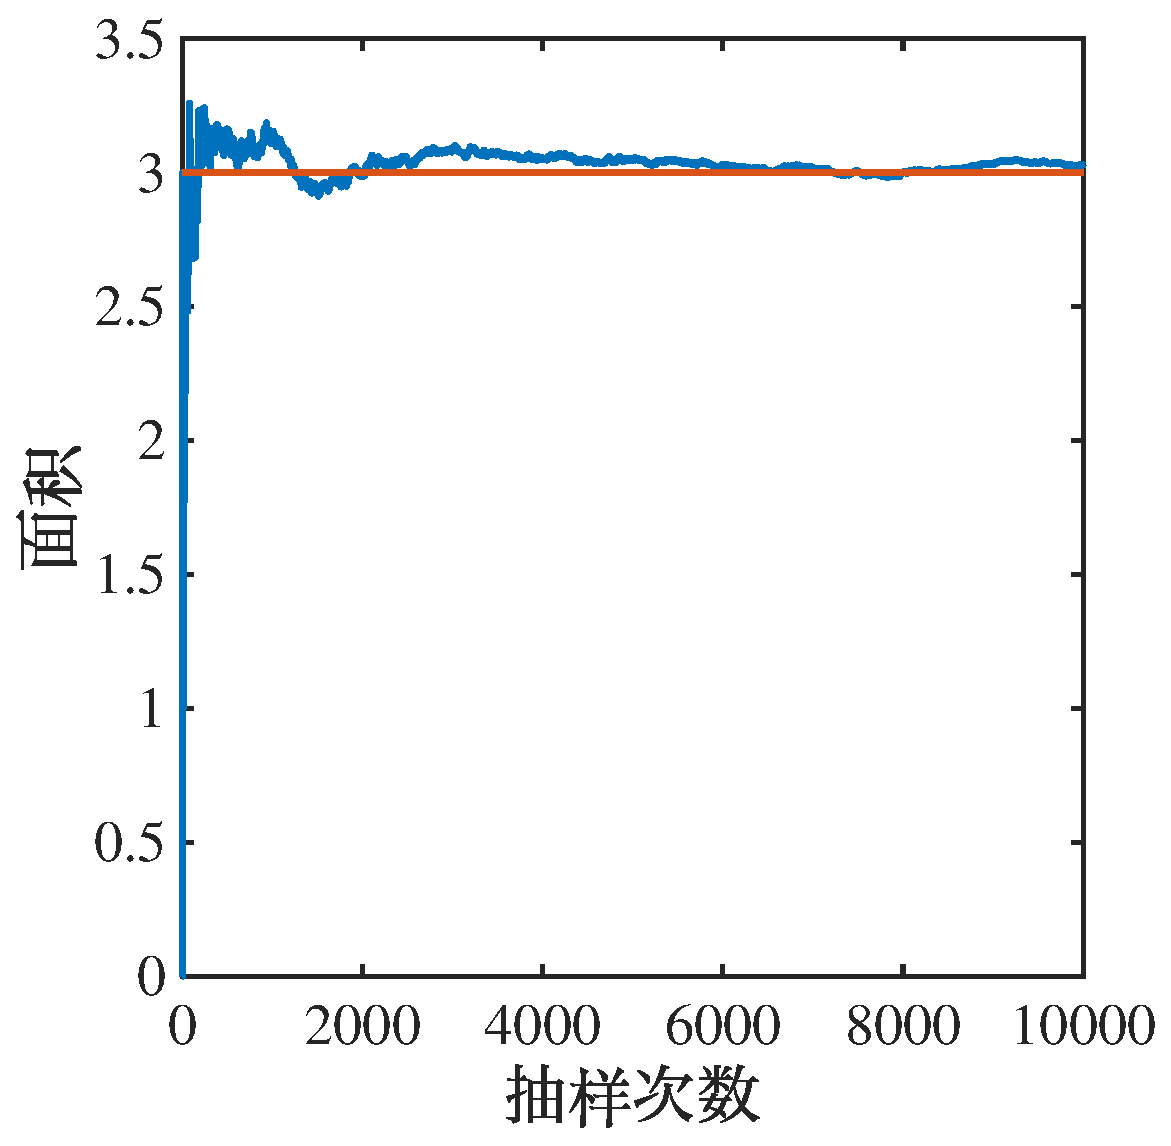
\includegraphics[width=7cm]{1.eps}
	\caption{简单抽样。}
	\label{fig:1}
\end{figure}

\begin{figure}[htp]
	\centering
	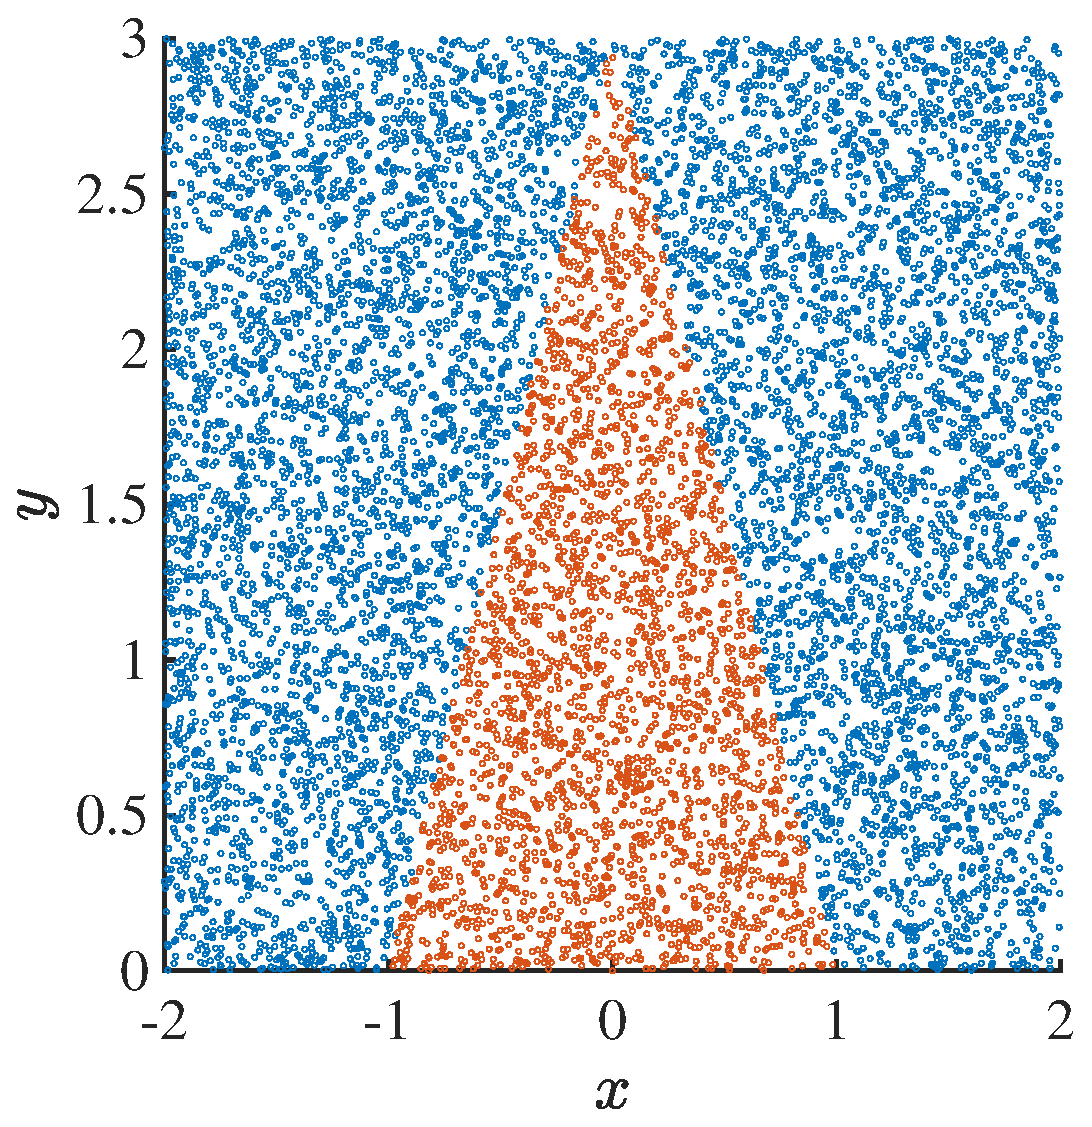
\includegraphics[width=7cm]{2.eps}
	\caption{简单抽样散点分布图。}
	\label{fig:2}
\end{figure}


\begin{figure}[htp]
	\centering
	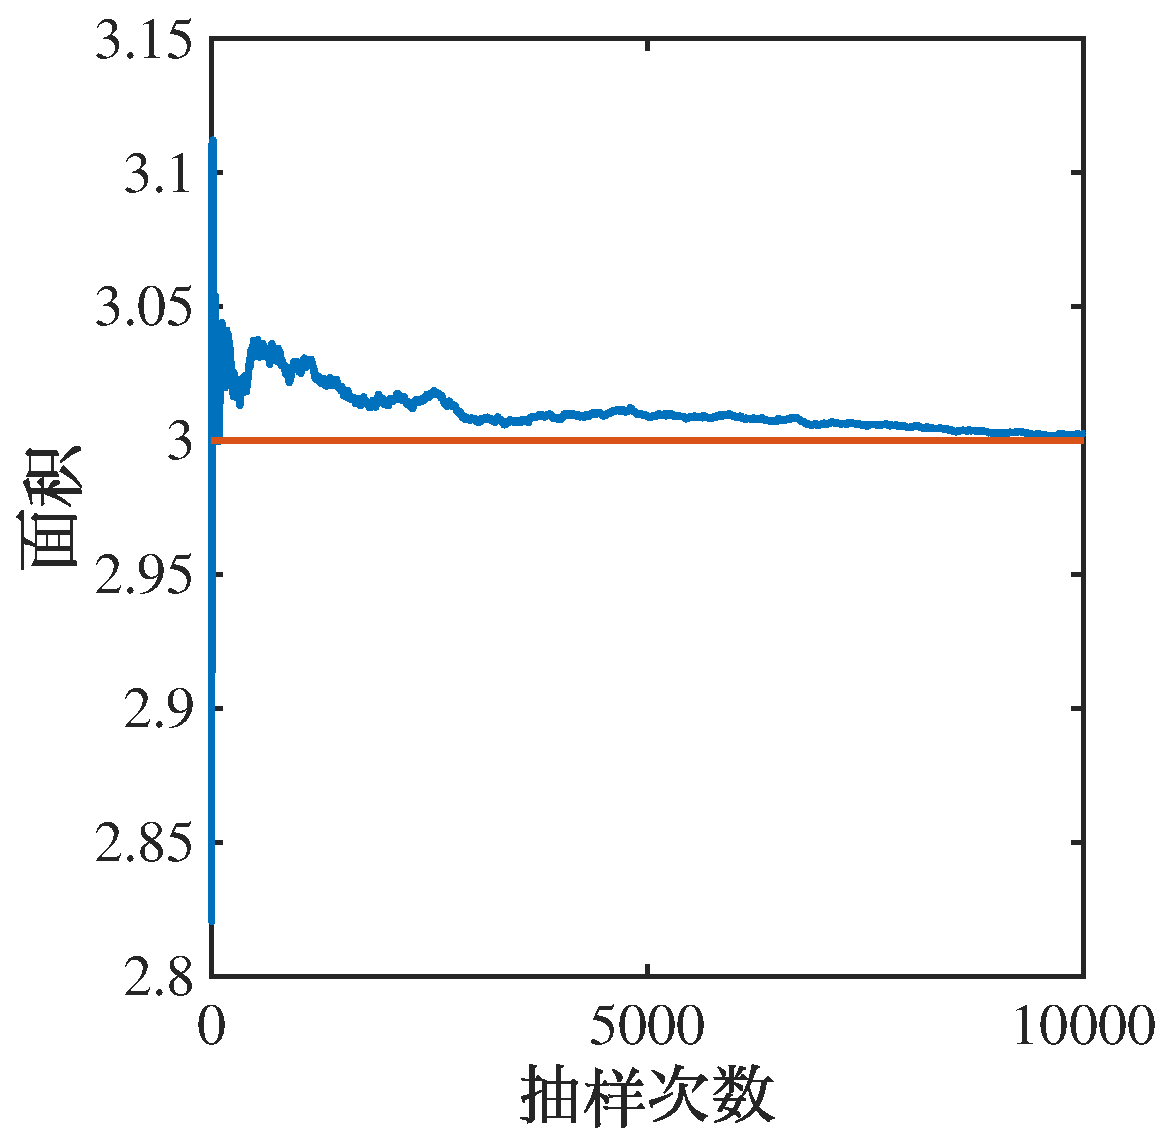
\includegraphics[width=7cm]{3.eps}
	\caption{重要抽样。}
	\label{fig:3}
\end{figure}


\begin{figure}[htp]
	\centering
	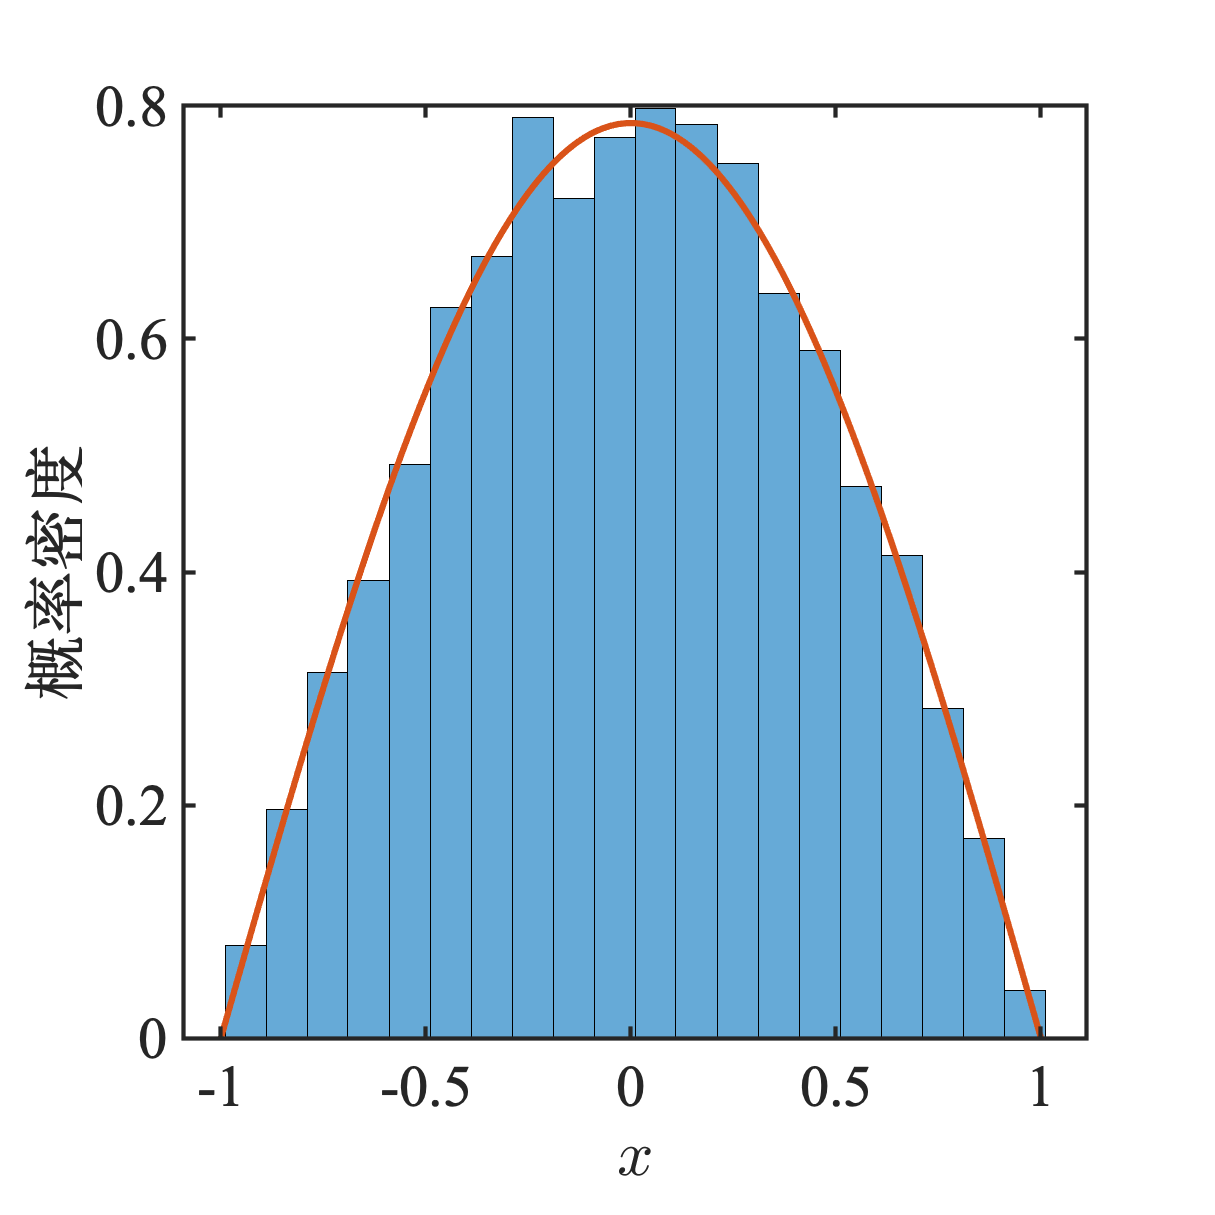
\includegraphics[width=7cm]{4.eps}
	\caption{$x$点的分布概率密度。}
	\label{fig:4}
\end{figure}


\begin{figure}[htp]
	\centering
	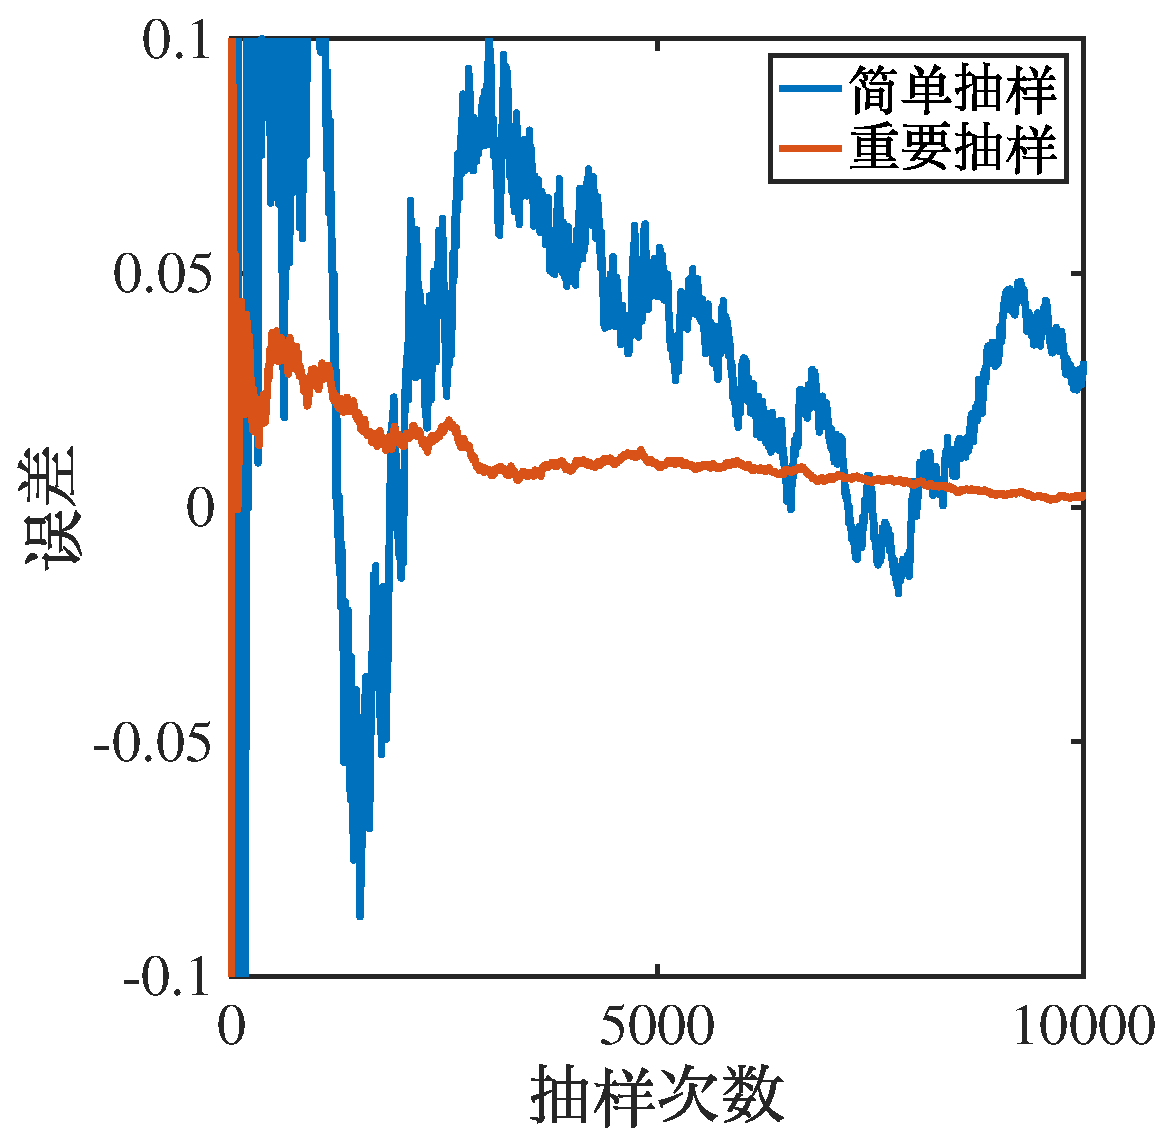
\includegraphics[width=7cm]{5.eps}
	\caption{两种方法的误差比较。}
	\label{fig:5}
\end{figure}

\section{态密度}

\subsection{转子的态密度}

考虑$\theta = \frac{\pi}{2}$的情况,
\begin{equation}
	\varepsilon = \frac{p^2_\varphi}{2I} = \frac{L^2}{2I}.
\end{equation}
其中
\begin{equation}
	I = m r^2.
\end{equation}

由不确定关系
\begin{equation}
	\Delta \varphi \Delta p_\varphi = h,
\end{equation}
又$\varphi\in [0,2\pi]$,例子可能的状态数为
\begin{equation}
	\frac{2\pi \dif p_\varphi}{h},
\end{equation}
所以态密度
\begin{equation}
	D(\varepsilon) \dif \varepsilon = \frac{\pi}{h} \sqrt{\frac{2I}{\varepsilon}}\dif \varepsilon.
\end{equation}


\subsection{氮分子的态密度}

考虑$\theta = \frac{\pi}{2}$的情况,
\begin{equation}
	\varepsilon = \frac{p^2_\varphi}{2I} = \frac{L^2}{2I}.
\end{equation}
其中
\begin{equation}
	I = m r^2.
\end{equation}

则
\begin{equation}
	\varepsilon = \frac{p^2}{2m} + \frac{1}{2} m \omega^2 x^2 + \frac{p^2_\varphi}{2I}.
\end{equation}
是一个椭球,三个轴的长度为
\begin{equation}
	a=\sqrt{2m\varepsilon},\quad b=\sqrt{\frac{2\varepsilon}{m \omega^2}},\quad c=\sqrt{2I\varepsilon},
\end{equation}
体积为
\begin{equation}
	V = \frac{4\pi}{3} abc.
\end{equation}
又,考虑到$\varphi$的积分为$2\pi$,以及不确定度为$h^2$
所以态密度
\begin{equation}
	D(\varepsilon) = \frac{2\pi}{h^2}\frac{\dif V}{\dif \varepsilon} = \frac{6\pi}{h^2\omega} \sqrt{2I\varepsilon}.
\end{equation}














% \nocite{*}

\newpage
\bibliographystyle{unsrtnat}

\phantomsection

\addcontentsline{toc}{section}{参考文献} %向目录中添加条目,以章的名义
\bibliography{homework}

\end{document}
